\section{Proofs of Construction}\label{sec:reasoning}

- approach to proving the correctness of our state channel network protocol

- the nature of state channels tends to make the logic complex
- value is moved between participants by exchanging statements about the distribution of assets held on-chain
- inevitably you end up reasoning about the statements you hold and their interpretation by the chain, and the possible actions of the other participants in the channel

- inherent danger, funds are locked on-chain
- participants act maliciously and stop cooperating at any point in the protocol
- safe at all times

\subsection{Channel Funding and Value}

We will start by considering the interpretation of the outcome of a state channel.
Suppose $A$ is a participant in a state channel, $L$, that reaches an (allocation) outcome, $\omega$, that allocates $x$ coins to $A$.
What does that mean for $A$?
In particular, how much more can $A$ withdraw from the system due to that outcome?
Understanding this is key to analysing state channel networks.

\begin{figure}[h]\centering
  \makebox[\textwidth][c]{\begin{tikzpicture}[node distance=0.3cm]
  \node (outcome) at (0, 0) {
    \begin{tikzpicture}[x=0.7cm]
      \node[circAB, label=right:$L$] (L) at (0, 0) {};
      \node[circA, label=below:$A$] (A) at (-1, -1) {};
      \node[circB, label=below:$B$] (B) at (1, -1) {};
      \draw[->] (L) edge node[midway, left] { $3$ } (A);
      \draw[->] (L) edge node[midway, right] { $4$ } (B);
    \end{tikzpicture}
  };
  \node[right=of outcome] (plus) {$+$};
  \node[right=of plus] (otherstuff) {$\dots$};
  \node[right=2cm of otherstuff] (balance) {
    \begin{tikzpicture}
      \node[sqadj] (adj) at (0, 0) {};
      \node[circA, label=below:$A$] (A) at (0, -1) {};
      \draw[->] (adj) edge node[midway, left] { $3$ } (A);
    \end{tikzpicture}
  };
  \draw[shorten <=0.5cm, shorten >=0.3cm, -{Latex[length=2mm]}] (otherstuff) edge node[midway, above] { ? } (balance);
  \node[right=of balance] (plus2) {$+$};
  \node[right=of plus2] {$\dots$};
\end{tikzpicture}
}
  \caption{
  }\label{fig:meaning-of-funding}
\end{figure}

There is one case where the answer to these questions is very straightforward:
where the channel $L$ itself has enough coins in the adjudicator to cover the entire allocation.
In this case, we say the channel is \textbf{directly funded}.
If this happens, $A$ will receive all $x$ coins allocated to them in $\omega$.
\begin{figure}[h]\centering
  \makebox[\textwidth][c]{\begin{tikzpicture}[node distance=2cm]
  \node (diag0) {
    \begin{tikzpicture}[y=1cm, x=2cm]
      \node[sqadj] (a0) at (1, 0) {};
      \node[circAB, label=right:$L$] (p0) at (1, -1) {};
      \node[circA, label=below:$A$] (p1) at (0.58, -2) {};
      \node[circB, label=below:$B$] (p2) at (1.42, -2) {};

      \draw[->] (a0) edge node[midway, left] { $7$ } (p0);
      \draw[->] (p0) edge node[midway, left] { $3$ } (p1);
      \draw[->] (p0) edge node[midway, right] { $4$ } (p2);

    \end{tikzpicture}
  };

  \node[right=of diag0] (diag1) {
    \begin{tikzpicture}[y=1cm, x=1.5cm]
      \node[sqadj] (a0) at (0, 0) {};
      \node[circA, label=below:$A$] (p0) at (0, -1) {};
      \draw[->] (a0) edge node[midway, left] { $3$ } (p0);

      \node[sqadj] (a1) at (1, 0) {};
      \node[circAB, label=right:L] (pab) at (1, -1) {};
      \node[circB, label=below:Bob] (pabb) at (1, -2) {};
      \draw[->] (a1) edge node[midway, left] { $4$ } (pab);
      \draw[->] (pab) edge node[midway, left] { $4$ } (pabb);
    \end{tikzpicture}
  };

  \draw[shorten <=0.5cm, shorten >=0.3cm, -{Latex[length=2mm]}] (diag0) to (diag1);
\end{tikzpicture}
}
  \caption{
  }\label{fig:direct-funding}
\end{figure}

This is a good start, but the whole point of state channel \textit{networks} is to move beyond the case where every channel needs to be directly funded.
Suppose instead that $L$ is not directly funded but there is another channel, $L'$, that is.
Further suppose that $L'$ has reached an outcome where all its coins are allocated to $L$.
Using this outcome, we know we can redistribute the coins in the adjudicator to $L$, recreating the situation above, where $L$ was directly funded.
In this situation we can also say that $A$ will receive the $x$ coins from the outcome of $L$.
Note that we did not actually need to perform the redistribution on-chain to reach this conclusion - we just needed to be able to reason that the outcome enabled us to.


\begin{figure}[h]\centering
  \makebox[\textwidth][c]{\begin{tikzpicture}[node distance=2cm]
  \node (diag0) {
    \begin{tikzpicture}[y=1cm, x=1.5cm]
      \node[sqadj] (a0) at (1, 1) {};
      \node[circAB, label=right:$L'$] (l0) at (1, 0) {};


      \node[circAB, label=right:$L'$] (l1) at (2, 0) {};
      \node[circAB, label=right:$L$] (p0) at (2, -1) {};

      \draw[->] (a0) edge node[midway, left] { $7$ } (l0);
      \draw[->] (l1) edge node[midway, left] { $7$ } (p0);

    \end{tikzpicture}
  };

  \node[right=of diag0] (diag1) {
    \begin{tikzpicture}[y=1cm, x=2cm]
      \node[sqadj] (a0) at (1, 1) {};
      \node[circAB, label=right:$L'$] (l0) at (1, 0) {};
      \node[circAB, label=right:$L$] (p0) at (1, -1) {};

      \draw[->] (a0) edge node[midway, left] { $7$ } (l0);
      \draw[->] (l0) edge node[midway, left] { $7$ } (p0);

    \end{tikzpicture}
  };

  \node[right=of diag1] (diag2) {
    \begin{tikzpicture}[y=1cm, x=1.5cm]
      \node[sqadj] (a0) at (0, 0) {};
      \node[circAB, label=below:$L$] (p0) at (0, -1) {};
      \draw[->] (a0) edge node[midway, left] { $7$ } (p0);
    \end{tikzpicture}
  };

  \path[draw=none] (diag0) -- node (b) {\Large $\equiv$ } (diag1);
  \draw[shorten <=0.5cm, shorten >=0.3cm, -{Latex[length=2mm]}] (diag1) to (diag2);
\end{tikzpicture}
}
  \caption{
  }\label{fig:indirect-funding}
\end{figure}

- so far we've been looking at outcomes
- but in a state channel we don't have outcomes
- we can see the state of the adjudicator: direct fundings, finalized outcomes
- we have some private information: private keys, secrets for the channel algorithm (e.g. our ship positions in a game of battleships)
- we have the statements we've received and the statements we've sent

\begin{figure}[h]\centering
  \makebox[\textwidth][c]{\begin{tikzpicture}[node distance=2cm]
  \node[cloud, draw,cloud puffs=10,cloud puff arc=120, aspect=2, inner ysep=1em, align=center] (systemstate) {$\Sigma$};

  \node[right=of systemstate] (diag0) {
    \begin{tikzpicture}[y=1cm, x=2cm]
      \node[sqadj] (a0) at (1, 0) {};
      \node[circAB, label=right:$L$] (p0) at (1, -1) {};
      \node[circA, label=below:$A$] (p1) at (0.58, -2) {};
      \node[circB, label=below:$B$] (p2) at (1.42, -2) {};

      \draw[->] (a0) edge node[midway, left] { $7$ } (p0);
      \draw[->] (p0) edge node[midway, left] { $3$ } (p1);
      \draw[->] (p0) edge node[midway, right] { $4$ } (p2);

    \end{tikzpicture}
  };

  \node[right=of diag0] (diag1) {
    \begin{tikzpicture}[y=1cm, x=1.5cm]
      \node[sqadj] (a0) at (0, 0) {};
      \node[circA, label=below:$A$] (p0) at (0, -1) {};
      \draw[->] (a0) edge node[midway, left] { $3$ } (p0);

      \node[sqadj] (a1) at (1, 0) {};
      \node[circAB, label=right:L] (pab) at (1, -1) {};
      \node[circB, label=below:Bob] (pabb) at (1, -2) {};
      \draw[->] (a1) edge node[midway, left] { $4$ } (pab);
      \draw[->] (pab) edge node[midway, left] { $4$ } (pabb);
    \end{tikzpicture}
  };

  \draw[shorten <=0.5cm, shorten >=0.3cm, -{Latex[length=2mm]}] (systemstate) to (diag0);
  \draw[shorten <=0.5cm, shorten >=0.3cm, -{Latex[length=2mm]}] (diag0) to (diag1);
\end{tikzpicture}
}
  \caption{
  }\label{fig:system-state-direct-funding}
\end{figure}

- definition of funding
- definition of value


\subsection{Constructing}

- 1. show that a given network funds a channel
- 2. show you can build it step-by-step

second point is important
- single channel updates
- keep that channels are independent - which allows us to reason about finalizability on a per channel basis

simple rule that you can transition between them if you have equal values

\subsection{Unbeatable Strategies}

- unbeatable strategy for obtaining a balance on-chain
- two parts: finalization and redistribution

- finalization is per channel - channels independent
- outcome isn't always determined
\begin{figure}[h]\centering
  \makebox[\textwidth][c]{\begin{tikzpicture}[x=5cm, y=2cm]
  \node[cloud, draw,cloud puffs=10,cloud puff arc=120, aspect=2, inner ysep=1em, align=center] (systemstate) at (0,0) {$\Sigma$};

  \node (opt0) at (1.2, 1) {
    \begin{tikzpicture}[y=1cm, x=2cm]
      \node[sqadj] (a0) at (1, 0) {};
      \node[circAB, label=right:$L$] (p0) at (1, -1) {};
      \node[circA, label=below:$A$] (p1) at (0.58, -2) {};
      \node[circB, label=below:$B$] (p2) at (1.42, -2) {};

      \draw[->] (a0) edge node[midway, left] { $7$ } (p0);
      \draw[->] (p0) edge node[midway, left] { $3$ } (p1);
      \draw[->] (p0) edge node[midway, right] { $4$ } (p2);

    \end{tikzpicture}
  };
   
  % \node (opt2) at (1, 0) {$\vdots$ };

  \node (opt1) at (0.9, -1) {
    \begin{tikzpicture}[y=1cm, x=0.82cm]
      \node[sqadj] (a0) at (1, 0) {};
      \node[circAB, label=right:$L$] (p0) at (1, -1) {};
      \node[circA, label=below:$A$] (p1) at (0, -2) {};
      \node[circAB, label=right:$L'$] (p2) at (2, -2) {};
      \node[circA, label=below:$A$] (p3) at (1, -3) {};
      \node[circB, label=below:$B$] (p4) at (3, -3) {};

      \draw[->] (a0) edge node[midway, left] { $7$ } (p0);
      \draw[->] (p0) edge node[midway, left] { $2$ } (p1);
      \draw[->] (p0) edge node[midway, right] { $5$ } (p2);
      \draw[->] (p2) edge node[midway, right] { $1$ } (p3);
      \draw[->] (p2) edge node[midway, right] { $4$ } (p4);

    \end{tikzpicture}
  };

  \node (val) at (2, 0) {
    \begin{tikzpicture}[y=1cm, x=1.5cm]
      \node[sqadj] (a0) at (0, 0) {};
      \node[circA, label=below:$A$] (p0) at (0, -1) {};
      \draw[->] (a0) edge node[midway, left] { $3$ } (p0);
    \end{tikzpicture}
  };

  \draw[shorten <=0.5cm, shorten >=0.3cm, -{Latex[length=2mm]}] (systemstate) to (opt0);
  \draw[shorten <=0.5cm, shorten >=0.3cm, -{Latex[length=2mm]}] (systemstate) to (opt1);
  % \draw[shorten <=0.5cm, shorten >=0.3cm, -{Latex[length=2mm]}] (systemstate) to (opt2);
  \draw[shorten <=0.5cm, shorten >=0.3cm, -{Latex[length=2mm]}] (opt0) to (val);
  \draw[shorten <=0.5cm, shorten >=0.3cm, -{Latex[length=2mm]}] (opt1) to (val);
  % \draw[shorten <=0.5cm, shorten >=0.3cm, -{Latex[length=2mm]}] (opt2) to (val);
\end{tikzpicture}
}
  \caption{Cool, huh?}
\end{figure}


- more in finalizable outcomes

- redistribution is hard
- need to consider all different possibilities
- develop tools for the protocol to argue about this
- will be done in the turbo / nitro section

- rules

\subsection{Finalizable Outcomes}

- definition in terms of unbeatable strategy

- example: next mover

- different possibilities
  - finalized

- universal finalizability
- two examples
- diagram: FM states
\begin{figure}[h]\centering
  \makebox[\textwidth][c]{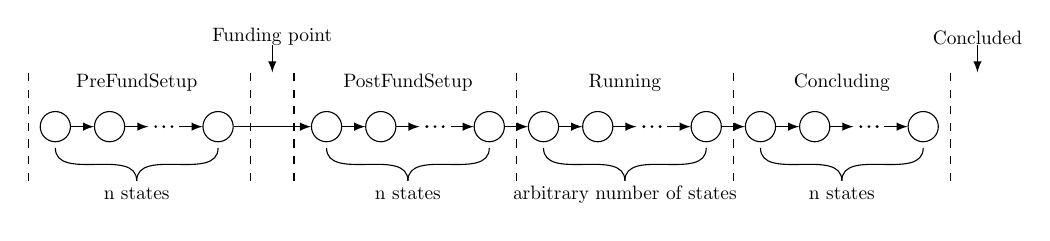
\begin{tikzpicture}[x=28pt,y=28pt,scale=0.7, every node/.style={transform shape}]
  \newcommand{\paperdiagram}[3]{%
    \begin{scope}[shift={(#1,0)}]
      % Circle
      \foreach \n in {0,1,3} {\node[circle,draw,text width=10pt,inner sep=0pt] (N\n#1) at (\n,0) {\strut};}
      % Transparent circle
      \foreach \n in {2} {\node[circle,draw,text width=10pt,inner sep=0pt,white] (N\n#1) at (\n,0) {\strut};}
      % Dots
      \foreach \n in {1.85,2,2.15} {\fill (\n,0) circle (0.8pt);}
      % Arrows
      \foreach \x [remember=\x as \lastx (initially 0)] in {1,2,3}{\draw[-latex] (N\lastx#1) -- (N\x#1);}
      % Under brackets with label #3
      \foreach \n in {0,3} {\draw ([shift={(0,-3pt)}]N\n#1.south) to[out=270,in=90] (1.5,-1) node[inner sep=1pt] (P) {\strut};}
      \node at (P.south) {\strut#3};
      % Upper label #2
      \node at (1.5,0.8) {\strut#2};
    \end{scope}
  }
  % Diagram nodes
  \paperdiagram{0}{PreFundSetup}{n states}
  \paperdiagram{5}{PostFundSetup}{n states}
  \paperdiagram{9}{Running}{arbitrary number of states}
  \paperdiagram{13}{Concluding}{n states}
  % Arrows between single diagram node
  \foreach \x [remember=\x as \lastx (initially 0)] in {5,9,13}{\draw[-latex] (N3\lastx) -- (N0\x);}
  % Vertical dashed
  \foreach \n in {-0.5,3.6,4.4,8.5,12.5,16.5} {\draw[dashed] (\n,-1) --++(90:2);}
  % Funding arrow
  \draw[latex-] (4,1) --++(90:0.5) node[at end,above,inner sep=0pt] {Funding point};
  \draw[latex-] (17,1) --++(90:0.5) node[at end,above,inner sep=0pt] {Concluded};
\end{tikzpicture}
}
  \caption{Cool, huh?}
\end{figure}

- enabled outcomes

\subsection{Consensus Game}

- consensus game if FM application
- deals in outcome. accepted outcome, propose a new one
- has the property that the only two possible outcomes are A and B
\begin{figure}[h]\centering
  \makebox[\textwidth][c]{\begin{tikzpicture}[x=1.7cm, y=1cm]
  \begin{scope}[every node/.style={draw,circle,minimum size=4mm}]
    \node (A) at (0,0) {};
    \node (AB1) at (1,0) {};
    \node (AB2) at (2,0) {};
    \node[draw=none] (ABx) at (3,0) {};
    % Dots
    \foreach \n in {2.95,3,3.05} {\fill (\n,0) circle (0.8pt);}
    \node (ABn) at (4,0) {};
    \node (B) at (5,0) {};
  \end{scope}
  \begin{scope}
    \node at ([yshift=-0.5cm]A) { $A$ };
    \node at ([yshift=-0.5cm]AB1) { $(A, B, 1)$ };
    \node at ([yshift=-0.5cm]AB2) { $(A, B, 2)$ };
    \node at ([yshift=-0.5cm]ABn) { $(A, B, n-1)$ };
    \node at ([yshift=-0.5cm]B) { $B$ };
  \end{scope}
  \begin{scope}[-{Latex[length=2mm]}]
    \draw (A) to (AB1);
    \draw (AB1) to (AB2);
    \draw (AB2) to (ABx);
    \draw (ABx) to (ABn);
    \draw (ABn) to (B);
    \draw (AB1) to[bend right] (A);
    \draw (AB2) to[bend right] (A);
    \draw (ABn) to[bend right] (A);
  \end{scope}
\end{tikzpicture}
}
  \caption{Cool, huh?}
\end{figure}

\subsection{Outcomes First}

- in practice it is hard to write states
- instead we will write outcomes and reason about when you can transition between them

- use special type of channel - consensus game channel


- if I have two network outcomes that differ in the outcome of a single CG channel
- then I can find a sequence of single-update network states that interpolate between them

- write down a sequence of outcomes
- update one channel at a time
- and have the same value to all participants

- the start and conclude states are also finalizable

\begin{figure}[h]\centering
  \makebox[\textwidth][c]{\begin{tikzpicture}[node distance=1cm]
  \node (s0) {
    \begin{tikzpicture}[x=0.7cm]
      \node[circAB, label=right:$L$] (L) at (0, 0) {};
      \node[circA, label=below:$A$] (A) at (-1, -1) {};
      \node[circB, label=below:$B$] (B) at (1, -1) {};
      \draw[->] (L) edge node[midway, left] { $3$ } (A);
      \draw[->] (L) edge node[midway, right] { $4$ } (B);
    \end{tikzpicture}
  };
  \node[right=of s0.south east, anchor=south west] (s1) {
    \begin{tikzpicture}[y=1cm, x=0.7cm]
      \node[sqadj] (a0) at (1, 0) {};
      \node[circAB, label=right:$L$] (p0) at (1, -1) {};
      \node[circA, label=below:$A$] (p1) at (0, -2) {};
      \node[circB, label=below:$B$] (p2) at (2, -2) {};

      \draw[->] (a0) edge node[midway, left] { $7$ } (p0);
      \draw[->] (p0) edge node[midway, left] { $3$ } (p1);
      \draw[->] (p0) edge node[midway, right] { $4$ } (p2);

    \end{tikzpicture}
  };

  \node[right=of s1.north east, anchor = north west] (s2) {
    \begin{tikzpicture}[y=1cm, x=2cm]
      \node[sqadj] (a0) at (1, 0) {};
      \node[circAB, label=right:$L$] (p0) at (1, -1) {};

      \draw[->] (a0) edge node[midway, left] { $7$ } (p0);

    \end{tikzpicture}
  };

  \node[right=of s2.north east, anchor=north west] (s3) {
    \begin{tikzpicture}[y=1cm, x=2cm]
      \node[sqadj] (a0) at (1, 0) {};
      \node[circAB, label=right:$L$] (p0) at (1, -1) {};
      \node[circA, label=below:$A$] (p1) at (0.58, -2) {};
      \node[circB, label=below:$B$] (p2) at (1.42, -2) {};

      \draw[->] (a0) edge node[midway, left] { $7$ } (p0);
      \draw[->] (p0) edge node[midway, left] { $6$ } (p1);
      \draw[->] (p0) edge node[midway, right] { $1$ } (p2);

    \end{tikzpicture}
  };

  \node[right=of s3.north east, anchor=north west] (s4) {
    \begin{tikzpicture}[y=1cm, x=1cm]
      \node[sqadj] (a0) at (1, 0) {};
      \node[circA, label=below:$A$] (p0) at (1, -1) {};
      \node[sqadj] (a1) at (2, 0) {};
      \node[circB, label=below:$B$] (p1) at (2, -1) {};

      \draw[->] (a0) edge node[midway, left] { $6$ } (p0);
      \draw[->] (a1) edge node[midway, left] { $1$ } (p1);

    \end{tikzpicture}
  };
  \node (mid) at ([yshift=-3mm] s0.north) {};
  \begin{scope}[-{Latex[length=2mm]}]
    \draw (s0.east |- mid) to (s1.west |- mid);
    \draw (s1.east |- mid) to (s2.west |- mid);
    \draw (s2.east |- mid) to (s3.west |- mid);
    \draw (s3.east |- mid) to (s4.west |- mid);
  \end{scope}

  \node[below=-1mm of s0] (below) { (a) };
  \node at (s1 |- below) { (b) };
  \node at (s2 |- below) { (c) };
  \node at (s3 |- below) { (d) };
  \node at (s4 |- below) { (e) };
\end{tikzpicture}
}
  \caption{Cool, huh?}
\end{figure}
